\documentclass{beamer}
\usepackage[utf8]{inputenc}

\usetheme{Madrid}
\usecolortheme{default}
\usepackage{amsmath,amssymb,amsfonts,amsthm}
\usepackage{txfonts}
\usepackage{tkz-euclide}
\usepackage{listings}
\usepackage{adjustbox}
\usepackage{array}
\usepackage{tabularx}
\usepackage{gvv}
\usepackage{lmodern}
\usepackage{circuitikz}
\usepackage{tikz}
\usepackage{graphicx}

\setbeamertemplate{page number in head/foot}[totalframumber]

\usepackage{tcolorbox}
\tcbuselibrary{minted,breakable,xparse,skins}



\definecolor{bg}{gray}{0.95}
\DeclareTCBListing{mintedbox}{O{}m!O{}}{%
  breakable=true,
  listing engine=minted,
  listing only,
  minted language=#2,
  minted style=default,
  minted options={%
    linenos,
    gobble=0,
    breaklines=true,
    breakafter=,,
    fontsize=\small,
    numbersep=8pt,
    #1},
  boxsep=0pt,
  left skip=0pt,
  right skip=0pt,
  left=25pt,
  right=0pt,
  top=3pt,
  bottom=3pt,
  arc=5pt,
  leftrule=0pt,
  rightrule=0pt,
  bottomrule=2pt,
  toprule=2pt,
  colback=bg,
  colframe=orange!70,
  enhanced,
  overlay={%
    \begin{tcbclipinterior}
    \fill[orange!20!white] (frame.south west) rectangle ([xshift=20pt]frame.north west);
    \end{tcbclipinterior}},
  #3,
}
\lstset{
    language=C,
    basicstyle=\ttfamily\small,
    keywordstyle=\color{blue},
    stringstyle=\color{orange},
    commentstyle=\color{green!60!black},
    numbers=left,
    numberstyle=\tiny\color{gray},
    breaklines=true,
    showstringspaces=false,
}
%------------------------------------------------------------
%This block of code defines the information to appear in the
%Title page
\title %optional
{1.4.17}
\date{August 28,2025}
%\subtitle{A short story}

\author % (optional)
{EE25BTECH11002 - Achat Parth Kalpesh}



\begin{document}


\frame{\titlepage}
\begin{frame}{Question}
Find the coordinates of the points of trisection \brak{\text{i.e. points dividing to three equal parts}} of the line segment joining the points $\vec{A}$ \brak{2,-2} and $\vec{B}$ \brak{-7,4}.
\end{frame}



\begin{frame}{Theoretical Solution}

Let the vectors for the given points $\vec{A}$ and $\vec{B}$ be
\begin{align}
    \vec{A}=\begin{myvec}{2\\-2}\end{myvec}, 
    \vec{B}=\begin{myvec}{-7\\4}\end{myvec}
\end{align}
Let the points of trisection be $\vec{P}$ and $\vec{Q}$. Point $\vec{P}$ divides the line segment AB in the ratio $1:2$, 
and point $\vec{Q}$ divides it in the ratio $2:1$.

We can use the internal division formula to find the coordinates of $\vec{P}$ and $\vec{Q}$

\end{frame}

\begin{frame}{Equation}
The internal division formula for a vector $\vec{R}$ that divides the line segment formed by vectors $\vec{A}$ and $\vec{B}$ in the ratio m:n is given by:
\begin{align}
    \vec{R}=\frac{m\vec{B}+n\vec{A}}{m+n}
\end{align}
\end{frame}
\begin{frame}{Theoretical Solution}
For the first point of trisection, $\vec{P}$ \brak{\text{ratio 1:2}}\\
Here, m=1 and n=2.
\begin{align}
    \vec{P}=\frac{1\times\begin{myvec}{-7 \\ 4}\end{myvec}+2\times\begin{myvec}{2\\-2}\end{myvec}}{1+2}
\end{align}
\begin{align}
    \vec{P} = \frac{1}{3} \begin{myvec}{-7+4 \\ 4-4}\end{myvec} = \frac{1}{3} \begin{myvec}{-3 \\ 0}\end{myvec} = \begin{myvec}{-1\\0}\end{myvec}
\end{align}
So, the coordinates of $\vec{P}$ are \brak{-1, 0}.
\end{frame}

\begin{frame}{Theoretical Solution}
For the second point of trisection, $\vec{Q}$ \brak{\text{ratio 2:1}} \\
Here, m=2 and n=1.
\begin{align}
    \vec{Q}=\frac{2\times\begin{myvec}{-7 \\ 4}\end{myvec}+1\times\begin{myvec}{2\\-2}\end{myvec}}{2+1}
\end{align}
\begin{align}
    \vec{Q} = \frac{1}{3} \begin{myvec}{-14+2 \\ 8-2}\end{myvec} = \frac{1}{3} \begin{myvec}{-12 \\ 6}\end{myvec} = \begin{myvec}{-4\\2}\end{myvec}
\end{align}
So, the coordinates of $\vec{Q}$ are \brak{-4, 2}.
\end{frame}

\begin{frame}[fragile]
    \frametitle{C code}
    \begin{lstlisting}
#include <stdio.h>
void section_formula(float *P, float *A, float *B, int m, int n, int k){
for (int i = 0; i < k ; i++) {
    P[i] = (m*B[i]+n*A[i])/(m+n);
}
}
    \end{lstlisting}
\end{frame}

\begin{frame}[fragile]
    \frametitle{Python Code}
    \begin{lstlisting}
import sys
import ctypes
import numpy as np
import matplotlib.pyplot as plt
c_lib = ctypes.CDLL('./formula.so')

c_lib.section_formula.argtypes = [
    ctypes.POINTER(ctypes.c_float),  
    ctypes.POINTER(ctypes.c_float),  
    ctypes.POINTER(ctypes.c_float),  
    ctypes.c_int,                    
    ctypes.c_int,                    
    ctypes.c_int                     
]
c_lib.section_formula.restype = None  
k = 2 
A = np.array([2, -2], dtype=np.float32)
B = np.array([-7, 4], dtype=np.float32)
    \end{lstlisting}
\end{frame}


\begin{frame}[fragile]
    \frametitle{Python Code}
    \begin{lstlisting}
P = np.zeros(k, dtype=np.float32)
Q = np.zeros(k, dtype=np.float32)

m = 1
n = 2
c_lib.section_formula(
    P.ctypes.data_as(ctypes.POINTER(ctypes.c_float)),
    A.ctypes.data_as(ctypes.POINTER(ctypes.c_float)),
    B.ctypes.data_as(ctypes.POINTER(ctypes.c_float)),
    m,
    n,
    k
)
m = 2
n = 1
    \end{lstlisting}
\end{frame}


\begin{frame}[fragile]
    \frametitle{Python Code}
    \begin{lstlisting}
c_lib.section_formula(
    Q.ctypes.data_as(ctypes.POINTER(ctypes.c_float)), 
    A.ctypes.data_as(ctypes.POINTER(ctypes.c_float)),
    B.ctypes.data_as(ctypes.POINTER(ctypes.c_float)),
    m,
    n,
    k
)
plt.plot([A[0], B[0]], [A[1], B[1]], label='Line AB', zorder=1)
all_points = np.vstack([A, B, P, Q])
plt.scatter(all_points[:, 0], all_points[:, 1], color='red', zorder=2)
vert_labels = ['A', 'B', 'P', 'Q']
for i, txt in enumerate(vert_labels):
    plt.annotate(f'{txt}\n({all_points[i, 0]:.1f}, {all_points[i, 1]:.1f})',
                 (all_points[i, 0], all_points[i, 1]),

    \end{lstlisting}
\end{frame}


\begin{frame}[fragile]
    \frametitle{Python Code}
    \begin{lstlisting}
                 textcoords="offset points", xytext=(0,10), ha='center')
ax = plt.gca()
ax.spines['left'].set_position('zero')
ax.spines['bottom'].set_position('zero')
ax.spines['right'].set_color('none')
ax.spines['top'].set_color('none')
plt.xlabel('$x$')
plt.ylabel('$y$')
plt.legend(loc='upper right')
plt.grid(True)
plt.axis('equal')
plt.savefig('plot_from_c_corrected.png')
plt.show()
    \end{lstlisting}
\end{frame}



\begin{frame}{Plot}
    \begin{figure}
        \centering
        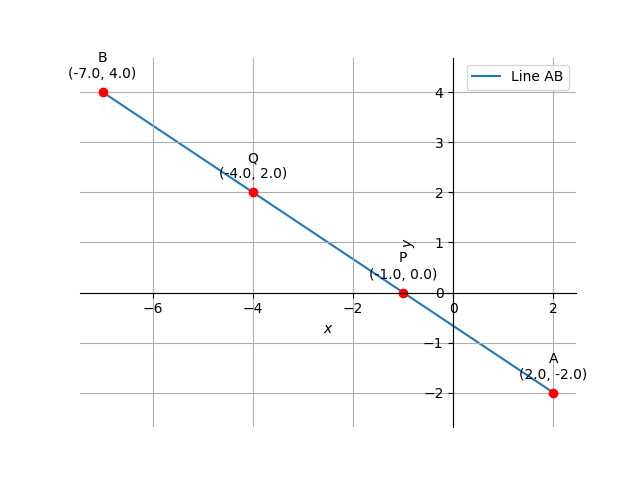
\includegraphics[width=0.5\columnwidth]{../figs/Plot_C.png}
        \caption{Trisection of the line segment joining $\vec{A}$ \brak{2,-2} and $\vec{B}$ \brak{-7,4}}
        \label{fig:fig}
    \end{figure}
\end{frame}






\end{document}









